\documentclass{beamer}

% Should be documentclass beamer

\mode<presentation>
{
%  \usetheme[hideothersubsections]{PaloAlto}
  \usetheme{metropolis}
  \setbeamercovered{transparent}
}

\input{commonm}

\newcommand{\hdr}[2]{
  \title[CS 5220, Fall 2017]{CS 5220: #2}
  \author{David Bindel}
  \institute{Cornell}
  \date{#1}
}


\hdr{2017-09-14}{Locality and parallelism in simulations II}


\begin{document}

\begin{frame}
  \titlepage
\end{frame}


\begin{frame}
  \frametitle{Basic styles of simulation}

  \begin{itemize}
  \item Discrete event systems (continuous or discrete time)
    \begin{itemize}
    \item Game of life, logic-level circuit simulation
    \item Network simulation
    \end{itemize}
  \item Particle systems
    \begin{itemize}
    \item Billiards, electrons, galaxies, ...
    \item Ants, cars, ...?
    \end{itemize}
  \item Lumped parameter models (ODEs)
    \begin{itemize}
    \item Circuits (SPICE), structures, chemical kinetics
    \end{itemize}
  \item Distributed parameter models (PDEs / integral equations)
    \begin{itemize}
    \item Heat, elasticity, electrostatics, ...
    \end{itemize}
  \end{itemize}
  Often more than one type of simulation appropriate. \\
  Sometimes more than one at a time!

\end{frame}


\begin{frame}
  \frametitle{Common ideas / issues}

  \begin{itemize}
  \item Load balancing
    \begin{itemize}
    \item Imbalance may be from lack of parallelism, poor distribution
    \item Can be static or dynamic
    \end{itemize}
  \item Locality
    \begin{itemize}
    \item Want big blocks with low surface-to-volume ratio
    \item Minimizes communication / computation ratio
    \item Can generalize ideas to graph setting
    \end{itemize}
  \item Tensions and tradeoffs
    \begin{itemize}
    \item Irregular spatial decompositions for load balance
      at the cost of complexity, maybe extra communication
    \item Particle-mesh methods --- can't manage moving particles
      and fixed meshes simultaneously without communicating
    \end{itemize}
  \end{itemize}

\end{frame}


\begin{frame}
  \frametitle{Lumped parameter simulations}

  Examples include:
  \begin{itemize}
  \item SPICE-level circuit simulation 
    \begin{itemize}
    \item nodal voltages vs. voltage distributions
    \end{itemize}
  \item Structural simulation 
    \begin{itemize}
    \item beam end displacements vs. continuum field
    \end{itemize}
  \item Chemical concentrations in stirred tank reactor
    \begin{itemize}
    \item concentrations in tank vs. spatially varying concentrations
    \end{itemize}
  \end{itemize}
  
  \vspace{5mm}
  Typically involves ordinary differential equations (ODEs), \\
  or with constraints (differential-algebraic equations, or DAEs).

  \vspace{5mm}
  Often (not always) {\em sparse}.
\end{frame}


\begin{frame}
  \frametitle{Sparsity}

  \begin{center}
    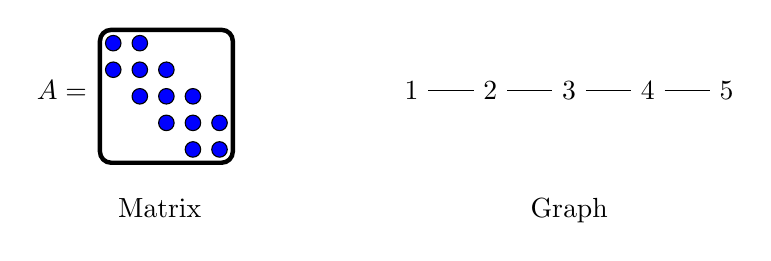
\begin{tikzpicture}

      % A = spy plot
      \draw (0,0.75) node[anchor=east] {$A=$};
      \begin{scope}[xshift=6pt,scale=2]
        \draw[ultra thick,rounded corners] (-2.40pt,21.60pt) rectangle (21.60pt,-2.40pt);
\draw[fill=blue] (0.00pt,19.20pt) circle [radius=1.4pt]; 
\draw[fill=blue] (4.80pt,19.20pt) circle [radius=1.4pt]; 
\draw[fill=blue] (0.00pt,14.40pt) circle [radius=1.4pt]; 
\draw[fill=blue] (4.80pt,14.40pt) circle [radius=1.4pt]; 
\draw[fill=blue] (9.60pt,14.40pt) circle [radius=1.4pt]; 
\draw[fill=blue] (4.80pt,9.60pt) circle [radius=1.4pt]; 
\draw[fill=blue] (9.60pt,9.60pt) circle [radius=1.4pt]; 
\draw[fill=blue] (14.40pt,9.60pt) circle [radius=1.4pt]; 
\draw[fill=blue] (9.60pt,4.80pt) circle [radius=1.4pt]; 
\draw[fill=blue] (14.40pt,4.80pt) circle [radius=1.4pt]; 
\draw[fill=blue] (19.20pt,4.80pt) circle [radius=1.4pt]; 
\draw[fill=blue] (14.40pt,0.00pt) circle [radius=1.4pt]; 
\draw[fill=blue] (19.20pt,0.00pt) circle [radius=1.4pt]; 

      \end{scope}

      % Graph picture
      \begin{scope}[xshift=4cm]
      \node (A) at (0,0.75) {1};
      \node (B) at (1,0.75) {2};
      \node (C) at (2,0.75) {3};
      \node (D) at (3,0.75) {4};
      \node (E) at (4,0.75) {5};
      \draw (A) -- (B) -- (C) -- (D) -- (E);
      \end{scope}

      \node[anchor=north] at (0.8,-0.5) {Matrix};
      \node[anchor=north] at (6,-0.5) {Graph};
    \end{tikzpicture}
  \end{center}

  Consider system of ODEs $x' = f(x)$ (special case: $f(x) = Ax$)
  \begin{itemize}
  \item 
    Dependency graph has edge $(i,j)$ if $f_j$ depends on $x_i$
  \item
    Sparsity means each $f_j$ depends on only a few $x_i$
  \item
    Often arises from physical or logical locality
  \item
    Corresponds to $A$ being a sparse matrix (mostly zeros)
  \end{itemize}
\end{frame}


\begin{frame}
  \frametitle{Sparsity and partitioning}

  \begin{center}
    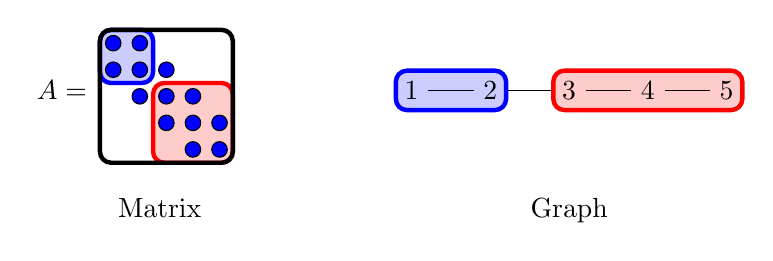
\begin{tikzpicture}


      % A = spy plot
      \draw (0,0.75) node[anchor=east] {$A=$};
      \begin{scope}[xshift=6pt,scale=2]
        \draw[ultra thick,rounded corners,color=blue,fill=blue!20] (-2.40pt,12.00pt) rectangle
        (7.20pt,21.60pt);
        \draw[ultra thick,rounded corners,color=red,fill=red!20] (7.20pt,12.00pt) rectangle
        (21.60pt,-2.40pt);

        \draw[ultra thick,rounded corners] (-2.40pt,21.60pt) rectangle (21.60pt,-2.40pt);
\draw[fill=blue] (0.00pt,19.20pt) circle [radius=1.4pt]; 
\draw[fill=blue] (4.80pt,19.20pt) circle [radius=1.4pt]; 
\draw[fill=blue] (0.00pt,14.40pt) circle [radius=1.4pt]; 
\draw[fill=blue] (4.80pt,14.40pt) circle [radius=1.4pt]; 
\draw[fill=blue] (9.60pt,14.40pt) circle [radius=1.4pt]; 
\draw[fill=blue] (4.80pt,9.60pt) circle [radius=1.4pt]; 
\draw[fill=blue] (9.60pt,9.60pt) circle [radius=1.4pt]; 
\draw[fill=blue] (14.40pt,9.60pt) circle [radius=1.4pt]; 
\draw[fill=blue] (9.60pt,4.80pt) circle [radius=1.4pt]; 
\draw[fill=blue] (14.40pt,4.80pt) circle [radius=1.4pt]; 
\draw[fill=blue] (19.20pt,4.80pt) circle [radius=1.4pt]; 
\draw[fill=blue] (14.40pt,0.00pt) circle [radius=1.4pt]; 
\draw[fill=blue] (19.20pt,0.00pt) circle [radius=1.4pt]; 

      \end{scope}

      % Graph picture
      \begin{scope}[xshift=4cm]
        \draw[ultra thick,rounded corners,color=blue,fill=blue!20]
          (-0.2,0.5) rectangle (1.2,1);
        \draw[ultra thick,rounded corners,color=red,fill=red!20]
          (1.8,0.5) rectangle (4.2,1);
        \node (A) at (0,0.75) {1};
        \node (B) at (1,0.75) {2};
        \node (C) at (2,0.75) {3};
        \node (D) at (3,0.75) {4};
        \node (E) at (4,0.75) {5};
        \draw (A) -- (B) -- (C) -- (D) -- (E);
      \end{scope}

      \node[anchor=north] at (0.8,-0.5) {Matrix};
      \node[anchor=north] at (6,-0.5) {Graph};
    \end{tikzpicture}
  \end{center}

  Want to partition sparse graphs so that
  \begin{itemize}
  \item Subgraphs are same size (load balance)
  \item Cut size is minimal (minimize communication)
  \end{itemize}
  We'll talk more about this later.

\end{frame}


\begin{frame}
  \frametitle{Types of analysis}
  
  Consider $x' = f(x)$ (special case: $f(x) = Ax + b$).  Might want:
  \begin{itemize}
  \item Static analysis ($f(x_*) = 0$)
    \begin{itemize}
    \item Boils down to $Ax = b$ (e.g. for Newton-like steps)
    \item Can solve directly or iteratively
    \item Sparsity matters a lot!
    \end{itemize}
  \item Dynamic analysis (compute $x(t)$ for many values of $t$)
    \begin{itemize}
    \item Involves time stepping (explicit or implicit)
    \item Implicit methods involve linear/nonlinear solves
    \item Need to understand stiffness and stability issues
    \end{itemize}
  \item Modal analysis (compute eigenvalues of $A$ or $f'(x_*)$)
  \end{itemize}

\end{frame}


\begin{frame}
  \frametitle{Explicit time stepping}
  
  \begin{itemize}
  \item Example: forward Euler
  \item Next step depends only on earlier steps
  \item Simple algorithms
  \item May have stability/stiffness issues
  \end{itemize}

\end{frame}


\begin{frame}
  \frametitle{Implicit time stepping}
  
  \begin{itemize}
  \item Example: backward Euler
  \item Next step depends on itself and on earlier steps
  \item Algorithms involve solves --- complication, communication!
  \item Larger time steps, each step costs more
  \end{itemize}

\end{frame}


\begin{frame}
  \frametitle{A common kernel}

  In all these analyses, spend lots of time in sparse matvec:
  \begin{itemize}
  \item Iterative linear solvers: repeated sparse matvec
  \item Iterative eigensolvers: repeated sparse matvec
  \item Explicit time marching: matvecs at each step
  \item Implicit time marching: iterative solves (involving matvecs)
  \end{itemize}
  We need to figure out how to make matvec fast!

\end{frame}

\begin{frame}
  \frametitle{An aside on sparse matrix storage}

  \begin{itemize}
  \item Sparse matrix $\implies$ mostly zero entries
    \begin{itemize}
    \item Can also have ``data sparseness'' --- representation with 
      less than $O(n^2)$ storage, even if most entries nonzero
    \end{itemize}
  \item Could be implicit (e.g. directional differencing)
  \item Sometimes explicit representation is useful
  \item Easy to get lots of indirect indexing!
  \item Compressed sparse storage schemes help
  \end{itemize}
\end{frame}


\begin{frame}
  \frametitle{Example: Compressed sparse row storage}

  \begin{center}
    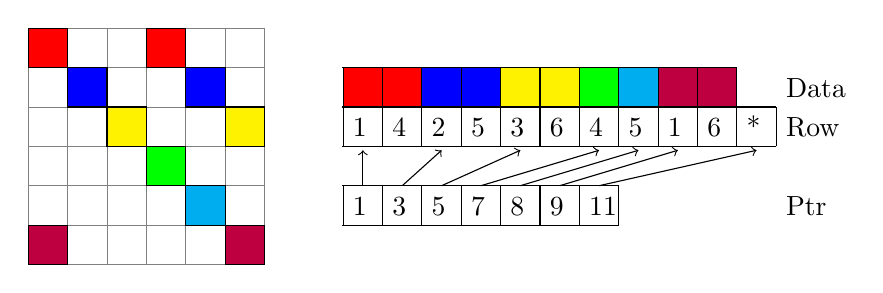
\begin{tikzpicture}
  \draw[step=0.5,gray,very thin] (-1,0) grid (2.0,3.0);
  \draw[fill=red]    (-1.0,2.5) rectangle (-0.5,3.0);
  \draw[fill=red]    ( 0.5,2.5) rectangle ( 1.0,3.0);
  \draw[fill=blue]   (-0.5,2.0) rectangle ( 0.0,2.5);
  \draw[fill=blue]   ( 1.0,2.0) rectangle ( 1.5,2.5);
  \draw[fill=yellow] ( 0.0,1.5) rectangle ( 0.5,2.0);
  \draw[fill=yellow] ( 1.5,1.5) rectangle ( 2.0,2.0);
  \draw[fill=green]  ( 0.5,1.0) rectangle ( 1.0,1.5);
  \draw[fill=cyan]   ( 1.0,0.5) rectangle ( 1.5,1.0);
  \draw[fill=purple] ( 1.5,0.0) rectangle ( 2.0,0.5);
  \draw[fill=purple] (-1.0,0.0) rectangle (-0.5,0.5);

  \draw[fill=red]    (3.0,2.0) rectangle (4.0,2.5);
  \draw[fill=blue]   (4.0,2.0) rectangle (5.0,2.5);
  \draw[fill=yellow] (5.0,2.0) rectangle (6.0,2.5);
  \draw[fill=green]  (6.0,2.0) rectangle (6.5,2.5);
  \draw[fill=cyan]   (6.5,2.0) rectangle (7.0,2.5);
  \draw[fill=purple] (7.0,2.0) rectangle (8.0,2.5);
  
  \draw[step=0.5,black] (2.99,2.0) grid (8.0,2.5);
  \draw[step=0.5,black] (2.99,1.499) grid (8.5,2.0);
  \draw[step=0.5,black] (2.99,0.499) grid (6.5,1.0);

  \draw (3.0,1.5) node[anchor=south west] {1};
  \draw (3.5,1.5) node[anchor=south west] {4};
  \draw (4.0,1.5) node[anchor=south west] {2};
  \draw (4.5,1.5) node[anchor=south west] {5};
  \draw (5.0,1.5) node[anchor=south west] {3};
  \draw (5.5,1.5) node[anchor=south west] {6};
  \draw (6.0,1.5) node[anchor=south west] {4};
  \draw (6.5,1.5) node[anchor=south west] {5};
  \draw (7.0,1.5) node[anchor=south west] {1};
  \draw (7.5,1.5) node[anchor=south west] {6};
  \draw (8.0,1.5) node[anchor=south west] {*};

  \draw (3.0,0.5) node[anchor=south west] {1};
  \draw (3.5,0.5) node[anchor=south west] {3};
  \draw (4.0,0.5) node[anchor=south west] {5};
  \draw (4.5,0.5) node[anchor=south west] {7};
  \draw (5.0,0.5) node[anchor=south west] {8};
  \draw (5.5,0.5) node[anchor=south west] {9};
  \draw (6.0,0.5) node[anchor=south west] {11};

  \draw [->] (3.25,1.0) -- (3.25,1.45); % 1
  \draw [->] (3.75,1.0) -- (4.25,1.45); % 3
  \draw [->] (4.25,1.0) -- (5.25,1.45); % 5
  \draw [->] (4.75,1.0) -- (6.25,1.45); % 7
  \draw [->] (5.25,1.0) -- (6.75,1.45); % 8
  \draw [->] (5.75,1.0) -- (7.25,1.45); % 9
  \draw [->] (6.25,1.0) -- (8.25,1.45);

  \draw (8.5,2.0) node[anchor=south west] {Data};
  \draw (8.5,1.5) node[anchor=south west] {Row};
  \draw (8.5,0.5) node[anchor=south west] {Ptr};
\end{tikzpicture}

  \end{center}
  
  This can be even more compact:
  \begin{itemize}
  \item Could organize by blocks (block CSR)
  \item Could compress column index data (16-bit vs 64-bit)
  \item Various other optimizations --- see OSKI
  \end{itemize}
\end{frame}


\begin{frame}
  \frametitle{Distributed parameter problems}

  Mostly PDEs:
  \begin{center}
  \begin{tabular}{llll}
    Type & Example & Time? & Space dependence? \\
    \hline
    Elliptic & electrostatics & steady & global \\
    Hyperbolic & sound waves & yes & local \\
    Parabolic  & diffusion   & yes & global
  \end{tabular}
  \end{center}

  \vspace{5mm}
  Different types involve different communication:
  \begin{itemize}
  \item Global dependence $\implies$ lots of communication \\
    (or tiny steps)
  \item Local dependence from finite wave speeds; \\
    limits communication
  \end{itemize}

\end{frame}


\begin{frame}
  \frametitle{Example: 1D heat equation}

  \begin{center}
    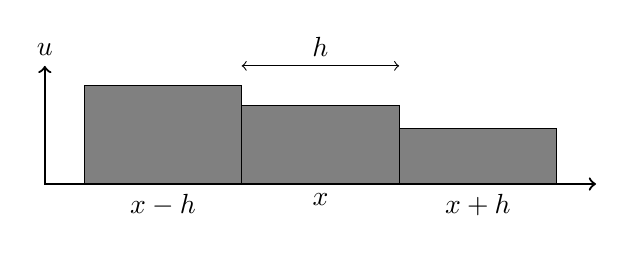
\begin{tikzpicture}
  \draw[<->,thick] (0,1.5) node[above] {$u$} |- (7,0);
  \draw[fill=gray] (0.5,0) rectangle (2.5,1.25);
  \draw[fill=gray] (2.5,0) rectangle (4.5,1.00);
  \draw[fill=gray] (4.5,0) rectangle (6.5,0.70);
  \draw[<->] (2.5,1.5) -- (4.5,1.5);
  \draw (3.5,1.5) node[anchor=south] {$h$};
  \draw (1.5,0) node[anchor=north] {$x-h$};
  \draw (3.5,0) node[anchor=north] {$x$};
  \draw (5.5,0) node[anchor=north] {$x+h$};
\end{tikzpicture}

  \end{center}

  Consider flow (e.g. of heat) in a uniform rod
  \begin{itemize}
  \item Heat ($Q$) $\propto$ 
    temperature ($u$) $\times$ mass ($\rho h$)
  \item Heat flow $\propto$ temperature gradient (Fourier's law)
  \end{itemize}

  \begin{align*}
     \frac{\partial Q}{\partial t} \propto
     h \frac{\partial u}{\partial t} &\approx
     C \left[ \left( \frac{u(x-h)-u(x)}{h} \right) +
              \left( \frac{u(x)-u(x+h)}{h} \right) \right] \\
    \frac{\partial u}{\partial t} &\approx
    C \left[ \frac{u(x-h)-2u(x)+u(x+h)}{h^2} \right] \rightarrow
    C \frac{\partial^2 u}{\partial x^2}
  \end{align*}
  
\end{frame}


\begin{frame}
  \frametitle{Spatial discretization}

  Heat equation with $u(0) = u(1) = 0$
  \[
  \frac{\partial u}{\partial t} = C \frac{\partial^2 u}{\partial x^2}
  \]

  Spatial semi-discretization:
  \[
  \frac{\partial^2 u}{\partial x^2} \approx \frac{u(x-h)-2u(x)+u(x+h)}{h^2}
  \]
  Yields a system of ODEs
  \[
  \frac{du}{dt} = C h^{-2} (-T) u =
  -C h^{-2}
  \begin{bmatrix}
     2 & -1      &   &    &        & \\
    -1 &  2      & -1 &    &        & \\
       & \ddots  & \ddots & \ddots & \\
       &         & -1      & 2     & -1 \\
       &         &        &  -1     & 2
  \end{bmatrix}
  \begin{bmatrix} u_1 \\ u_2 \\ \vdots \\ u_{n-2} \\ u_{n-1} \end{bmatrix}
  \]
\end{frame}


\begin{frame}
  \frametitle{Explicit time stepping}

  Approximate PDE by ODE system (``method of lines''):
  \[
    \frac{du}{dt} = C h^{-2} T u
  \]
  Now need a time-stepping scheme for the ODE:
  \begin{itemize}
  \item Simplest scheme is Euler:
    \[
      u(t+\delta) \approx u(t) + u'(t) \delta
                  = \left( I - C \frac{\delta}{h^2} T \right) u(t)
    \]
  \item Taking a time step $\equiv$ sparse matvec with
    $\left( I - C \frac{\delta}{h^2} T \right)$
  \item This may not end well...
  \end{itemize}

\end{frame}


\begin{frame}
  \frametitle{Explicit time stepping data dependence}

  \begin{center}
    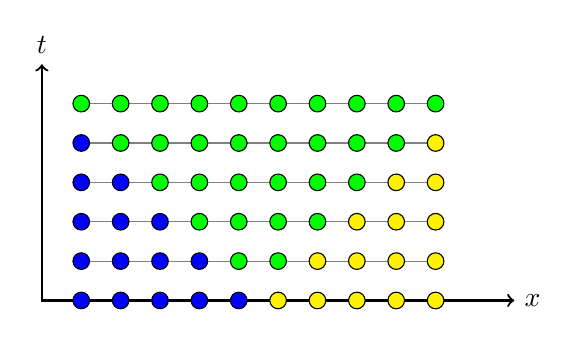
\begin{tikzpicture}
  \draw[<->,thick] (0,3) node[anchor=south] {$t$}
                |- (6,0) node[anchor=west] {$x$};

  \draw[fill=blue]   (0.5,0) circle (3pt);
  \draw[fill=blue]   (1.0,0) circle (3pt);
  \draw[fill=blue]   (1.5,0) circle (3pt);
  \draw[fill=blue]   (2.0,0) circle (3pt);
  \draw[fill=blue]   (2.5,0) circle (3pt);
  \draw[fill=yellow] (3.0,0) circle (3pt);
  \draw[fill=yellow] (3.5,0) circle (3pt);
  \draw[fill=yellow] (4.0,0) circle (3pt);
  \draw[fill=yellow] (4.5,0) circle (3pt);
  \draw[fill=yellow] (5.0,0) circle (3pt);

  \draw[thin,gray]   (0.5,0.5) -- (5.0,0.5);
  \draw[fill=blue]   (0.5,0.5) circle (3pt);
  \draw[fill=blue]   (1.0,0.5) circle (3pt);
  \draw[fill=blue]   (1.5,0.5) circle (3pt);
  \draw[fill=blue]   (2.0,0.5) circle (3pt);
  \draw[fill=green]  (2.5,0.5) circle (3pt);
  \draw[fill=green]  (3.0,0.5) circle (3pt);
  \draw[fill=yellow] (3.5,0.5) circle (3pt);
  \draw[fill=yellow] (4.0,0.5) circle (3pt);
  \draw[fill=yellow] (4.5,0.5) circle (3pt);
  \draw[fill=yellow] (5.0,0.5) circle (3pt);
  
  \draw[thin,gray]   (0.5,1.0) -- (5.0,1.0);
  \draw[fill=blue]   (0.5,1.0) circle (3pt);
  \draw[fill=blue]   (1.0,1.0) circle (3pt);
  \draw[fill=blue]   (1.5,1.0) circle (3pt);
  \draw[fill=green]  (2.0,1.0) circle (3pt);
  \draw[fill=green]  (2.5,1.0) circle (3pt);
  \draw[fill=green]  (3.0,1.0) circle (3pt);
  \draw[fill=green]  (3.5,1.0) circle (3pt);
  \draw[fill=yellow] (4.0,1.0) circle (3pt);
  \draw[fill=yellow] (4.5,1.0) circle (3pt);
  \draw[fill=yellow] (5.0,1.0) circle (3pt);

  \draw[thin,gray]   (0.5,1.5) -- (5.0,1.5);
  \draw[fill=blue]   (0.5,1.5) circle (3pt);
  \draw[fill=blue]   (1.0,1.5) circle (3pt);
  \draw[fill=green]  (1.5,1.5) circle (3pt);
  \draw[fill=green]  (2.0,1.5) circle (3pt);
  \draw[fill=green]  (2.5,1.5) circle (3pt);
  \draw[fill=green]  (3.0,1.5) circle (3pt);
  \draw[fill=green]  (3.5,1.5) circle (3pt);
  \draw[fill=green]  (4.0,1.5) circle (3pt);
  \draw[fill=yellow] (4.5,1.5) circle (3pt);
  \draw[fill=yellow] (5.0,1.5) circle (3pt);

  \draw[thin,gray]   (0.5,2.0) -- (5.0,2.0);      
  \draw[fill=blue]   (0.5,2.0) circle (3pt);
  \draw[fill=green]  (1.0,2.0) circle (3pt);
  \draw[fill=green]  (1.5,2.0) circle (3pt);
  \draw[fill=green]  (2.0,2.0) circle (3pt);
  \draw[fill=green]  (2.5,2.0) circle (3pt);
  \draw[fill=green]  (3.0,2.0) circle (3pt);
  \draw[fill=green]  (3.5,2.0) circle (3pt);
  \draw[fill=green]  (4.0,2.0) circle (3pt);
  \draw[fill=green]  (4.5,2.0) circle (3pt);
  \draw[fill=yellow] (5.0,2.0) circle (3pt);

  \draw[thin,gray]   (0.5,2.5) -- (5.0,2.5);      
  \draw[fill=green]  (0.5,2.5) circle (3pt);
  \draw[fill=green]  (1.0,2.5) circle (3pt);
  \draw[fill=green]  (1.5,2.5) circle (3pt);
  \draw[fill=green]  (2.0,2.5) circle (3pt);
  \draw[fill=green]  (2.5,2.5) circle (3pt);
  \draw[fill=green]  (3.0,2.5) circle (3pt);
  \draw[fill=green]  (3.5,2.5) circle (3pt);
  \draw[fill=green]  (4.0,2.5) circle (3pt);
  \draw[fill=green]  (4.5,2.5) circle (3pt);
  \draw[fill=green]  (5.0,2.5) circle (3pt);

\end{tikzpicture}

  \end{center}
  \begin{center}
    Nearest neighbor interactions per step $\implies$ \\
    finite rate of numerical information propagation
  \end{center}

\end{frame}


\begin{frame}[fragile]
  \frametitle{Explicit time stepping in parallel}
  
  \begin{center}
    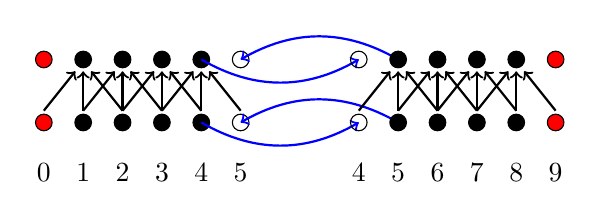
\begin{tikzpicture}
  \draw[fill=red]   (0.0,-0.2) node[anchor=north] {0};
  \draw[fill=black] (0.5,-0.2) node[anchor=north] {1};
  \draw[fill=black] (1.0,-0.2) node[anchor=north] {2};
  \draw[fill=black] (1.5,-0.2) node[anchor=north] {3};
  \draw[fill=black] (2.0,-0.2) node[anchor=north] {4};
  \draw             (2.5,-0.2) node[anchor=north] {5};
  
  \draw             (4.0,-0.2) node[anchor=north] {4};
  \draw[fill=black] (4.5,-0.2) node[anchor=north] {5};
  \draw[fill=black] (5.0,-0.2) node[anchor=north] {6};
  \draw[fill=black] (5.5,-0.2) node[anchor=north] {7};
  \draw[fill=black] (6.0,-0.2) node[anchor=north] {8};
  \draw[fill=red]   (6.5,-0.2) node[anchor=north] {9};
  
  \draw[fill=red]   (0.0,0.2) circle (3pt);
  \draw[fill=black] (0.5,0.2) circle (3pt);
  \draw[fill=black] (1.0,0.2) circle (3pt);
  \draw[fill=black] (1.5,0.2) circle (3pt);
  \draw[fill=black] (2.0,0.2) circle (3pt);
  \draw             (2.5,0.2) circle (3pt);

  \draw[thick,blue,->] (2.0,0.2) to [out=-30,in=210] (4.0,0.2);
  \draw[thick,blue,->] (4.5,0.2) to [out=150,in=30] (2.5,0.2);
  
  \draw             (4.0,0.2) circle (3pt);
  \draw[fill=black] (4.5,0.2) circle (3pt);
  \draw[fill=black] (5.0,0.2) circle (3pt);
  \draw[fill=black] (5.5,0.2) circle (3pt);
  \draw[fill=black] (6.0,0.2) circle (3pt);
  \draw[fill=red]   (6.5,0.2) circle (3pt);

  \draw[fill=red]   (0.0,1.0) circle (3pt);
  \draw[fill=black] (0.5,1.0) circle (3pt);
  \draw[fill=black] (1.0,1.0) circle (3pt);
  \draw[fill=black] (1.5,1.0) circle (3pt);
  \draw[fill=black] (2.0,1.0) circle (3pt);
  \draw             (2.5,1.0) circle (3pt);

  \draw[thick,blue,->] (2.0,1.0) to [out=-30,in=210] (4.0,1.0);
  \draw[thick,blue,->] (4.5,1.0) to [out=150,in=30]  (2.5,1.0);
        
  \draw             (4.0,1.0) circle (3pt);
  \draw[fill=black] (4.5,1.0) circle (3pt);
  \draw[fill=black] (5.0,1.0) circle (3pt);
  \draw[fill=black] (5.5,1.0) circle (3pt);
  \draw[fill=black] (6.0,1.0) circle (3pt);
  \draw[fill=red]   (6.5,1.0) circle (3pt);

  \draw[->,thick] (0.0,0.35) -- (0.4,0.85);
  \draw[->,thick] (0.5,0.35) -- (0.9,0.85);
  \draw[->,thick] (1.0,0.35) -- (1.4,0.85);
  \draw[->,thick] (1.5,0.35) -- (1.9,0.85);
  \draw[->,thick] (0.5,0.35) -- (0.5,0.85);
  \draw[->,thick] (1.0,0.35) -- (1.0,0.85);
  \draw[->,thick] (1.5,0.35) -- (1.5,0.85);
  \draw[->,thick] (2.0,0.35) -- (2.0,0.85);
  \draw[->,thick] (1.0,0.35) -- (0.6,0.85);
  \draw[->,thick] (1.5,0.35) -- (1.1,0.85);
  \draw[->,thick] (2.0,0.35) -- (1.6,0.85);
  \draw[->,thick] (2.5,0.35) -- (2.1,0.85);

  \draw[->,thick] (4.0,0.35) -- (4.4,0.85);
  \draw[->,thick] (4.5,0.35) -- (4.9,0.85);
  \draw[->,thick] (5.0,0.35) -- (5.4,0.85);
  \draw[->,thick] (5.5,0.35) -- (5.9,0.85);
  \draw[->,thick] (4.5,0.35) -- (4.5,0.85);
  \draw[->,thick] (5.0,0.35) -- (5.0,0.85);
  \draw[->,thick] (5.5,0.35) -- (5.5,0.85);
  \draw[->,thick] (6.0,0.35) -- (6.0,0.85);
  \draw[->,thick] (5.0,0.35) -- (4.6,0.85);
  \draw[->,thick] (5.5,0.35) -- (5.1,0.85);
  \draw[->,thick] (6.0,0.35) -- (5.6,0.85);
  \draw[->,thick] (6.5,0.35) -- (6.1,0.85);

\end{tikzpicture}

  \end{center}
\begin{verbatim}
for t = 1 to N
  communicate boundary data ("ghost cell")
  take time steps locally
end
\end{verbatim}

\end{frame}


\begin{frame}[fragile]
  \frametitle{Overlapping communication with computation}
  
  \begin{center}
    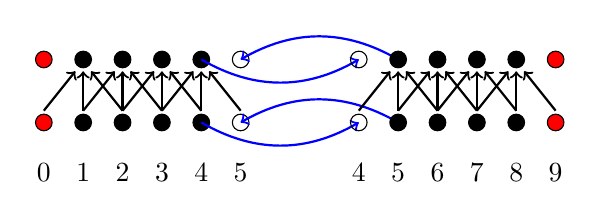
\begin{tikzpicture}
  \draw[fill=red]   (0.0,-0.2) node[anchor=north] {0};
  \draw[fill=black] (0.5,-0.2) node[anchor=north] {1};
  \draw[fill=black] (1.0,-0.2) node[anchor=north] {2};
  \draw[fill=black] (1.5,-0.2) node[anchor=north] {3};
  \draw[fill=black] (2.0,-0.2) node[anchor=north] {4};
  \draw             (2.5,-0.2) node[anchor=north] {5};
  
  \draw             (4.0,-0.2) node[anchor=north] {4};
  \draw[fill=black] (4.5,-0.2) node[anchor=north] {5};
  \draw[fill=black] (5.0,-0.2) node[anchor=north] {6};
  \draw[fill=black] (5.5,-0.2) node[anchor=north] {7};
  \draw[fill=black] (6.0,-0.2) node[anchor=north] {8};
  \draw[fill=red]   (6.5,-0.2) node[anchor=north] {9};
  
  \draw[fill=red]   (0.0,0.2) circle (3pt);
  \draw[fill=black] (0.5,0.2) circle (3pt);
  \draw[fill=black] (1.0,0.2) circle (3pt);
  \draw[fill=black] (1.5,0.2) circle (3pt);
  \draw[fill=black] (2.0,0.2) circle (3pt);
  \draw             (2.5,0.2) circle (3pt);

  \draw[thick,blue,->] (2.0,0.2) to [out=-30,in=210] (4.0,0.2);
  \draw[thick,blue,->] (4.5,0.2) to [out=150,in=30] (2.5,0.2);
  
  \draw             (4.0,0.2) circle (3pt);
  \draw[fill=black] (4.5,0.2) circle (3pt);
  \draw[fill=black] (5.0,0.2) circle (3pt);
  \draw[fill=black] (5.5,0.2) circle (3pt);
  \draw[fill=black] (6.0,0.2) circle (3pt);
  \draw[fill=red]   (6.5,0.2) circle (3pt);

  \draw[fill=red]   (0.0,1.0) circle (3pt);
  \draw[fill=black] (0.5,1.0) circle (3pt);
  \draw[fill=black] (1.0,1.0) circle (3pt);
  \draw[fill=black] (1.5,1.0) circle (3pt);
  \draw[fill=black] (2.0,1.0) circle (3pt);
  \draw             (2.5,1.0) circle (3pt);

  \draw[thick,blue,->] (2.0,1.0) to [out=-30,in=210] (4.0,1.0);
  \draw[thick,blue,->] (4.5,1.0) to [out=150,in=30]  (2.5,1.0);
        
  \draw             (4.0,1.0) circle (3pt);
  \draw[fill=black] (4.5,1.0) circle (3pt);
  \draw[fill=black] (5.0,1.0) circle (3pt);
  \draw[fill=black] (5.5,1.0) circle (3pt);
  \draw[fill=black] (6.0,1.0) circle (3pt);
  \draw[fill=red]   (6.5,1.0) circle (3pt);

  \draw[->,thick] (0.0,0.35) -- (0.4,0.85);
  \draw[->,thick] (0.5,0.35) -- (0.9,0.85);
  \draw[->,thick] (1.0,0.35) -- (1.4,0.85);
  \draw[->,thick] (1.5,0.35) -- (1.9,0.85);
  \draw[->,thick] (0.5,0.35) -- (0.5,0.85);
  \draw[->,thick] (1.0,0.35) -- (1.0,0.85);
  \draw[->,thick] (1.5,0.35) -- (1.5,0.85);
  \draw[->,thick] (2.0,0.35) -- (2.0,0.85);
  \draw[->,thick] (1.0,0.35) -- (0.6,0.85);
  \draw[->,thick] (1.5,0.35) -- (1.1,0.85);
  \draw[->,thick] (2.0,0.35) -- (1.6,0.85);
  \draw[->,thick] (2.5,0.35) -- (2.1,0.85);

  \draw[->,thick] (4.0,0.35) -- (4.4,0.85);
  \draw[->,thick] (4.5,0.35) -- (4.9,0.85);
  \draw[->,thick] (5.0,0.35) -- (5.4,0.85);
  \draw[->,thick] (5.5,0.35) -- (5.9,0.85);
  \draw[->,thick] (4.5,0.35) -- (4.5,0.85);
  \draw[->,thick] (5.0,0.35) -- (5.0,0.85);
  \draw[->,thick] (5.5,0.35) -- (5.5,0.85);
  \draw[->,thick] (6.0,0.35) -- (6.0,0.85);
  \draw[->,thick] (5.0,0.35) -- (4.6,0.85);
  \draw[->,thick] (5.5,0.35) -- (5.1,0.85);
  \draw[->,thick] (6.0,0.35) -- (5.6,0.85);
  \draw[->,thick] (6.5,0.35) -- (6.1,0.85);

\end{tikzpicture}

  \end{center}
\begin{verbatim}
for t = 1 to N
  start boundary data sendrecv
  compute new interior values
  finish sendrecv
  compute new boundary values
end
\end{verbatim}

\end{frame}



\begin{frame}[fragile]
  \frametitle{Batching time steps}

  \begin{center}
    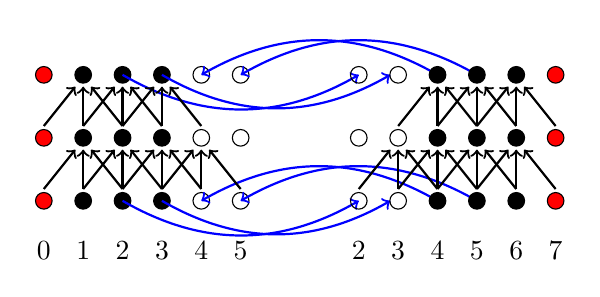
\begin{tikzpicture}
  \draw[fill=red]   (0.0,-0.2) node[anchor=north] {0};
  \draw[fill=black] (0.5,-0.2) node[anchor=north] {1};
  \draw[fill=black] (1.0,-0.2) node[anchor=north] {2};
  \draw[fill=black] (1.5,-0.2) node[anchor=north] {3};
  \draw             (2.0,-0.2) node[anchor=north] {4};
  \draw             (2.5,-0.2) node[anchor=north] {5};
  
  \draw             (4.0,-0.2) node[anchor=north] {2};
  \draw             (4.5,-0.2) node[anchor=north] {3};
  \draw[fill=black] (5.0,-0.2) node[anchor=north] {4};
  \draw[fill=black] (5.5,-0.2) node[anchor=north] {5};
  \draw[fill=black] (6.0,-0.2) node[anchor=north] {6};
  \draw[fill=red]   (6.5,-0.2) node[anchor=north] {7};
  
  \draw[fill=red]   (0.0,0.2) circle (3pt);
  \draw[fill=black] (0.5,0.2) circle (3pt);
  \draw[fill=black] (1.0,0.2) circle (3pt);
  \draw[fill=black] (1.5,0.2) circle (3pt);
  \draw             (2.0,0.2) circle (3pt);
  \draw             (2.5,0.2) circle (3pt);

  \draw[thick,blue,->] (1.0,0.2) to [out=-30,in=210] (4.0,0.2);
  \draw[thick,blue,->] (1.5,0.2) to [out=-30,in=210] (4.4,0.2);
  \draw[thick,blue,->] (5.0,0.2) to [out=150,in=30]  (2.0,0.2);
  \draw[thick,blue,->] (5.5,0.2) to [out=150,in=30]  (2.5,0.2);
  
  \draw             (4.0,0.2) circle (3pt);
  \draw             (4.5,0.2) circle (3pt);
  \draw[fill=black] (5.0,0.2) circle (3pt);
  \draw[fill=black] (5.5,0.2) circle (3pt);
  \draw[fill=black] (6.0,0.2) circle (3pt);
  \draw[fill=red]   (6.5,0.2) circle (3pt);

  \draw[fill=red]   (0.0,1.0) circle (3pt);
  \draw[fill=black] (0.5,1.0) circle (3pt);
  \draw[fill=black] (1.0,1.0) circle (3pt);
  \draw[fill=black] (1.5,1.0) circle (3pt);
  \draw             (2.0,1.0) circle (3pt);
  \draw             (2.5,1.0) circle (3pt);

  % \draw[thick,blue,->] (1.0,1.0) to [out=-30,in=210] (4.0,1.0);
  % \draw[thick,blue,->] (1.5,1.0) to [out=-30,in=210] (4.4,1.0);
  % \draw[thick,blue,->] (5.0,1.0) to [out=150,in=30]  (2.0,1.0);
  % \draw[thick,blue,->] (5.5,1.0) to [out=150,in=30]  (2.5,1.0);
        
  \draw             (4.0,1.0) circle (3pt);
  \draw             (4.5,1.0) circle (3pt);
  \draw[fill=black] (5.0,1.0) circle (3pt);
  \draw[fill=black] (5.5,1.0) circle (3pt);
  \draw[fill=black] (6.0,1.0) circle (3pt);
  \draw[fill=red]   (6.5,1.0) circle (3pt);

  \draw[fill=red]   (0.0,1.8) circle (3pt);
  \draw[fill=black] (0.5,1.8) circle (3pt);
  \draw[fill=black] (1.0,1.8) circle (3pt);
  \draw[fill=black] (1.5,1.8) circle (3pt);
  \draw             (2.0,1.8) circle (3pt);
  \draw             (2.5,1.8) circle (3pt);

  \draw[thick,blue,->] (1.0,1.8) to [out=-30,in=210] (4.0,1.8);
  \draw[thick,blue,->] (1.5,1.8) to [out=-30,in=210] (4.4,1.8);
  \draw[thick,blue,->] (5.0,1.8) to [out=150,in=30]  (2.0,1.8);
  \draw[thick,blue,->] (5.5,1.8) to [out=150,in=30]  (2.5,1.8);
        
  \draw             (4.0,1.8) circle (3pt);
  \draw             (4.5,1.8) circle (3pt);
  \draw[fill=black] (5.0,1.8) circle (3pt);
  \draw[fill=black] (5.5,1.8) circle (3pt);
  \draw[fill=black] (6.0,1.8) circle (3pt);
  \draw[fill=red]   (6.5,1.8) circle (3pt);

  \draw[->,thick] (0.0,0.35) -- (0.4,0.85);
  \draw[->,thick] (0.5,0.35) -- (0.9,0.85);
  \draw[->,thick] (1.0,0.35) -- (1.4,0.85);
  \draw[->,thick] (1.5,0.35) -- (1.9,0.85);
  \draw[->,thick] (0.5,0.35) -- (0.5,0.85);
  \draw[->,thick] (1.0,0.35) -- (1.0,0.85);
  \draw[->,thick] (1.5,0.35) -- (1.5,0.85);
  \draw[->,thick] (2.0,0.35) -- (2.0,0.85);
  \draw[->,thick] (1.0,0.35) -- (0.6,0.85);
  \draw[->,thick] (1.5,0.35) -- (1.1,0.85);
  \draw[->,thick] (2.0,0.35) -- (1.6,0.85);
  \draw[->,thick] (2.5,0.35) -- (2.1,0.85);

  \draw[->,thick] (4.0,0.35) -- (4.4,0.85);
  \draw[->,thick] (4.5,0.35) -- (4.9,0.85);
  \draw[->,thick] (5.0,0.35) -- (5.4,0.85);
  \draw[->,thick] (5.5,0.35) -- (5.9,0.85);
  \draw[->,thick] (4.5,0.35) -- (4.5,0.85);
  \draw[->,thick] (5.0,0.35) -- (5.0,0.85);
  \draw[->,thick] (5.5,0.35) -- (5.5,0.85);
  \draw[->,thick] (6.0,0.35) -- (6.0,0.85);
  \draw[->,thick] (5.0,0.35) -- (4.6,0.85);
  \draw[->,thick] (5.5,0.35) -- (5.1,0.85);
  \draw[->,thick] (6.0,0.35) -- (5.6,0.85);
  \draw[->,thick] (6.5,0.35) -- (6.1,0.85);

  \draw[->,thick] (0.0,1.15) -- (0.4,1.65);
  \draw[->,thick] (0.5,1.15) -- (0.9,1.65);
  \draw[->,thick] (1.0,1.15) -- (1.4,1.65);
%  \draw[->,thick] (1.5,1.15) -- (1.9,1.65);
  \draw[->,thick] (0.5,1.15) -- (0.5,1.65);
  \draw[->,thick] (1.0,1.15) -- (1.0,1.65);
  \draw[->,thick] (1.5,1.15) -- (1.5,1.65);
%  \draw[->,thick] (2.0,1.15) -- (2.0,1.65);
  \draw[->,thick] (1.0,1.15) -- (0.6,1.65);
  \draw[->,thick] (1.5,1.15) -- (1.1,1.65);
  \draw[->,thick] (2.0,1.15) -- (1.6,1.65);

  \draw[->,thick] (4.5,1.15) -- (4.9,1.65);
  \draw[->,thick] (5.0,1.15) -- (5.4,1.65);
  \draw[->,thick] (5.5,1.15) -- (5.9,1.65);
  \draw[->,thick] (5.0,1.15) -- (5.0,1.65);
  \draw[->,thick] (5.5,1.15) -- (5.5,1.65);
  \draw[->,thick] (6.0,1.15) -- (6.0,1.65);
  \draw[->,thick] (5.5,1.15) -- (5.1,1.65);
  \draw[->,thick] (6.0,1.15) -- (5.6,1.65);
  \draw[->,thick] (6.5,1.15) -- (6.1,1.65);

\end{tikzpicture}

  \end{center}
\begin{verbatim}
for t = 1 to N by B
  start boundary data sendrecv (B values)
  compute new interior values
  finish sendrecv (B values)
  compute new boundary values
end
\end{verbatim}

\end{frame}


\begin{frame}
  \frametitle{Explicit pain}

  \begin{center}
    \includegraphics[width=0.8\textwidth]{figs/explicit-unstable-demo.pdf} \\
    
    \vspace{5mm}
    Unstable for $\delta > O(h^2)$!
  \end{center}
  
\end{frame}


\begin{frame}
  \frametitle{Implicit time stepping}

  \begin{itemize}
  \item Backward Euler uses backward difference for $d/dt$
    \[
      u(t+\delta) \approx u(t) + u'(t + \delta t) \delta
    \]
  \item Taking a time step $\equiv$ sparse matvec with
    $\left( I + C \frac{\delta}{h^2} T \right)^{-1}$
  \item No time step restriction for stability (good!)
  \item But each step involves linear solve (not so good!)
    \begin{itemize}
    \item Good if you like numerical linear algebra?
    \end{itemize}
  \end{itemize}

\end{frame}


\begin{frame}
  \frametitle{Explicit and implicit}

  Explicit:
  \begin{itemize}
  \item Propagates information at finite rate
  \item Steps look like sparse matvec (in linear case)
  \item Stable step determined by fastest time scale
  \item Works fine for {\em hyperbolic} PDEs
  \end{itemize}

  Implicit:
  \begin{itemize}
  \item No need to resolve fastest time scales
  \item Steps can be long... but expensive
    \begin{itemize}
    \item Linear/nonlinear solves at each step
    \item Often these solves involve sparse matvecs
    \end{itemize}
  \item Critical for parabolic PDEs
  \end{itemize}
\end{frame}


\begin{frame}
  \frametitle{Poisson problems}

  Consider 2D Poisson
  \[
  -\nabla^2 u = 
    \frac{\partial^2 u}{\partial x^2} + 
    \frac{\partial^2 u}{\partial y^2} = f
  \]

  \begin{itemize}
  \item Prototypical elliptic problem (steady state)
  \item Similar to a backward Euler step on heat equation
  \end{itemize}
\end{frame}


\begin{frame}
  \frametitle{Poisson problem discretization}

  \begin{center}
%    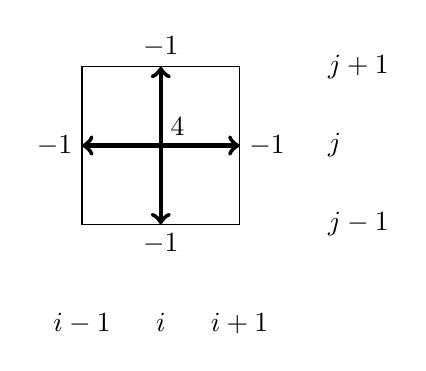
\begin{tikzpicture}
  \draw (0,0) rectangle (2,2);
  \draw [<->, ultra thick] (1,0) -- (1,2);
  \draw [<->, ultra thick] (0,1) -- (2,1);
  
  \node at (1,0) [below] {$-1$};
  \node at (1,2) [above] {$-1$};
  \node at (0,1) [left]  {$-1$};
  \node at (2,1) [right] {$-1$};
  \node at (1,1) [above right] {$4$};
  
  \node at (0,-1) [below] {$i-1$};
  \node at (1,-1) [below] {$i$};
  \node at (2,-1) [below] {$i+1$};

  \node at (3,0) [right] {$j-1$};
  \node at (3,1) [right] {$j$};
  \node at (3,2) [right] {$j+1$};
\end{tikzpicture}
 \\
  $
    u_{i,j} = h^{-2} \left( 4u_{i,j}-u_{i-1,j}-u_{i+1,j}-u_{i,j-1}-u_{i,j+1} \right)
  $
  \end{center}

  \[
  L =
  \left[
  \begin{array}{ccc|ccc|ccc}
     4 & -1 &    & -1 &    &    &    &    &    \\
    -1 &  4 & -1 &    & -1 &    &    &    &    \\
       & -1 &  4 &    &    & -1 &    &    &    \\ \hline
    -1 &    &    &  4 & -1 &    & -1 &    &    \\
       & -1 &    & -1 &  4 & -1 &    & -1 &    \\
       &    & -1 &    & -1 &  4 &    &    & -1 \\ \hline
       &    &    & -1 &    &    &  4 & -1 &    \\
       &    &    &    & -1 &    & -1 &  4 & -1 \\
       &    &    &    &    & -1 &    & -1 &  4 
  \end{array}
  \right]
  \]
\end{frame}


\begin{frame}
  \frametitle{Poisson solvers in 2D/3D}

  $N = n^d = $ total unknowns
  \vspace{2mm}

  \begin{tabular}{l|ll}
    Method & Time & Space \\ \hline
    Dense LU     & $N^3$          & $N^2$ \\
    Band LU      & $N^2$ ($N^{7/3}$) & $N^{3/2}$ ($N^{5/3}$) \\
    Jacobi       & $N^2$          & $N$ \\
    Explicit inv & $N^2$          & $N^2$ \\
    CG           & $N^{3/2}$       & $N$ \\
    Red-black SOR & $N^{3/2}$      & $N$ \\
    Sparse LU    & $N^{3/2}$       & $N \log N$ ($N^{4/3}$) \\
    FFT         & $N \log N$       & $N$ \\
    Multigrid   & $N$              & $N$
  \end{tabular}

  \vspace{5mm}
  Ref: Demmel, {\em Applied Numerical Linear Algebra}, SIAM, 1997.
  
  \vspace{5mm}
  Remember: best MFlop/s $\neq$ fastest solution!

\end{frame}


\begin{frame}
  \frametitle{General implicit picture}

  \begin{itemize}
  \item Implicit solves or steady state $\implies$ solving systems
  \item Nonlinear solvers generally linearize
  \item Linear solvers can be
    \begin{itemize}
    \item Direct (hard to scale)
    \item Iterative (often problem-specific)
    \end{itemize}
  \item Iterative solves boil down to matvec!
  \end{itemize}
\end{frame}


\begin{frame}
  \frametitle{PDE solver summary}
  
  \begin{itemize}
  \item Can be implicit or explicit (as with ODEs)
    \begin{itemize}
    \item Explicit (sparse matvec) --- fast, but short steps?
      \begin{itemize}
      \item works fine for hyperbolic PDEs
      \end{itemize}
    \item Implicit (sparse solve)
      \begin{itemize}
      \item Direct solvers are hard!
      \item Sparse solvers turn into matvec again
      \end{itemize}
    \end{itemize}
  \item Differential operators turn into local mesh stencils
    \begin{itemize}
    \item Matrix connectivity looks like mesh connectivity
    \item Can partition into subdomains that communicate only through
      boundary data
    \item More on graph partitioning later
    \end{itemize}
  \item Not all nearest neighbor ops are equally efficient!
    \begin{itemize}
    \item Depends on mesh structure
    \item Also depends on flops/point
    \end{itemize}
  \end{itemize}
\end{frame}


\end{document}
